\documentclass[12pt,letterpaper]{article}

\usepackage[utf8]{inputenc}
\usepackage[spanish]{babel}
\usepackage{amsmath}
\usepackage{amssymb}
\usepackage[left=2.5cm,right=2.5cm,top=2.5cm,bottom=2.5cm]{geometry}
\usepackage{listings}
\usepackage{xcolor}
\usepackage{graphicx}
\usepackage{hyperref}
\usepackage{booktabs}
\usepackage{lmodern}

% Configuración para bloques de código
\definecolor{codegreen}{rgb}{0,0.6,0}
\definecolor{codegray}{rgb}{0.5,0.5,0.5}
\definecolor{codepurple}{rgb}{0.58,0,0.82}
\definecolor{backcolour}{rgb}{0.95,0.95,0.92}

\lstdefinestyle{mystyle}{
    backgroundcolor=\color{backcolour},   
    commentstyle=\color{codegreen},
    keywordstyle=\color{magenta},
    numberstyle=\tiny\color{codegray},
    stringstyle=\color{codepurple},
    basicstyle=\ttfamily\footnotesize,
    breakatwhitespace=false,         
    breaklines=true,                 
    captionpos=b,                    
    keepspaces=true,                 
    numbers=left,                    
    numbersep=5pt,                  
    showspaces=false,                
    showstringspaces=false,
    showtabs=false,                  
    tabsize=2
}
\lstset{style=mystyle}

\title{\textbf{Reporte Técnico: Bucle de Cambio de Fase (Grokking) y Densificación de Variedad en el VAE}}
\author{Proyecto MIT - UNAL, Medellín \\ Hackathon Digital Twin}
\date{\today}

\begin{document}

\maketitle

\section{Introducción}
Este reporte presenta el desarrollo metodológico y los resultados de las tareas adicionales especificadas en el documento \texttt{Modificación.pdf}. Estas tareas complementan la recolección inicial mediante la exploración sistemática de la capacidad de generalización del Autoencoder Variacional (VAE) y el diseño de una estrategia de muestreo local gaussiano en regiones del espacio de búsqueda de alta transmisión iónica.

El objetivo fundamental es asegurar la solidez estadística y la eficiencia de datos de nuestro modelo, abordando directamente las métricas de evaluación de la hackathon:
\begin{itemize}
    \item \textbf{Eficiencia de datos (Rúbrica F):} Aprender la representación más rica posible con un número limitado de muestras físicas.
    \item \textbf{Exactitud en región informativa (Rúbrica A):} Enriquecer localmente el dataset donde ocurren impactos del haz de iones en el detector.
    \item \textbf{Admisibilidad física (Rúbrica G):} Asegurar que el espacio latente reconstruya perfiles de haz físicamente plausibles.
\end{itemize}

\section{Detección del Cambio de Fase (Grokking) en el VAE}
El concepto de \textit{Grokking} en el contexto del aprendizaje profundo se refiere al fenómeno donde un modelo transiciona de un estado de sobreajuste y memorización local de ruido a un estado de generalización suave y comprensión de las reglas físicas subyacentes, al incrementarse el número de muestras del dataset de entrenamiento.

\subsection{Bucle de Evaluación Experimental}
Para demostrar empíricamente esta transición de fase en el VAE, se implementó un bucle experimental estructurado bajo la siguiente secuencia lógica:
\begin{enumerate}
    \item \textbf{Set de Validación Fijo:} Se separaron de forma rígida $N_{\text{val}} = 30$ muestras obtenidas mediante Latin Hypercube Sampling (LHS) que nunca son expuestas durante la optimización del modelo.
    \item \textbf{Barrido de Tamaño de Entrenamiento ($N$):} Se iteró sobre el conjunto maestro de LHS tomando tamaños de subconjuntos de entrenamiento progresivos:
    \begin{equation}
        N \in [50,\, 100,\, 150,\, 200,\, 250,\, 300]
    \end{equation}
    \item \textbf{Re-inicialización de Pesos:} En cada paso $N$, los pesos y bias de la red VAE se reinician desde cero para asegurar una comparación justa y no sesgada por el historial previo de entrenamiento.
    \item \textbf{Entrenamiento del VAE:} Se entrena el modelo por $E = 150$ épocas utilizando la función de pérdida combinada de la evidencia inferior (\textit{ELBO}):
    \begin{equation}
        \mathcal{L}_{\text{VAE}} = \mathcal{L}_{\text{Recon}} + \beta \cdot \mathcal{L}_{\text{KL}}
    \end{equation}
    Donde $\mathcal{L}_{\text{Recon}}$ es la entropía cruzada binaria (BCE) sobre los bins normalizados en $[0,1]$ y $\mathcal{L}_{\text{KL}}$ es la divergencia de Kullback-Leibler con peso $\beta = 0.005$ para promover la suavidad en el espacio latente $z \in \mathbb{R}^2$.
    \item \textbf{Evaluación en Validación:} Al finalizar cada ciclo, se calcula el Error de Reconstrucción mediante el Error Cuadrático Medio (MSE) en el Set de Validación Fijo:
    \begin{equation}
        \text{MSE}_{\text{val}} = \frac{1}{M \cdot D} \sum_{i=1}^{M} \|X_i - \hat{X}_i\|_2^2
    \end{equation}
    Donde $M = 30$ y $D = 400$ bins.
\end{enumerate}

\subsection{Detección del Punto Crítico $N_c$}
Para determinar el "codo" de la curva de validación sin apelar a inspecciones visuales manuales, se programó un algoritmo basado en la proyección ortogonal. Dadas las coordenadas $\{(N_i, \text{MSE}_i)\}$, el algoritmo encuentra el punto que maximiza la distancia perpendicular hacia la línea recta (cuerda) que conecta el primer y el último punto experimental. El punto de máxima distancia se define como el punto crítico de transición de fase $N_c$.

\section{Resultados y Visualización de la Transición de Fase}
El bucle experimental se ejecutó con éxito. La gráfica generada de pérdida de validación en función de $N$ se almacena en el directorio de figuras del proyecto.

\begin{figure}[htbp]
    \centering
    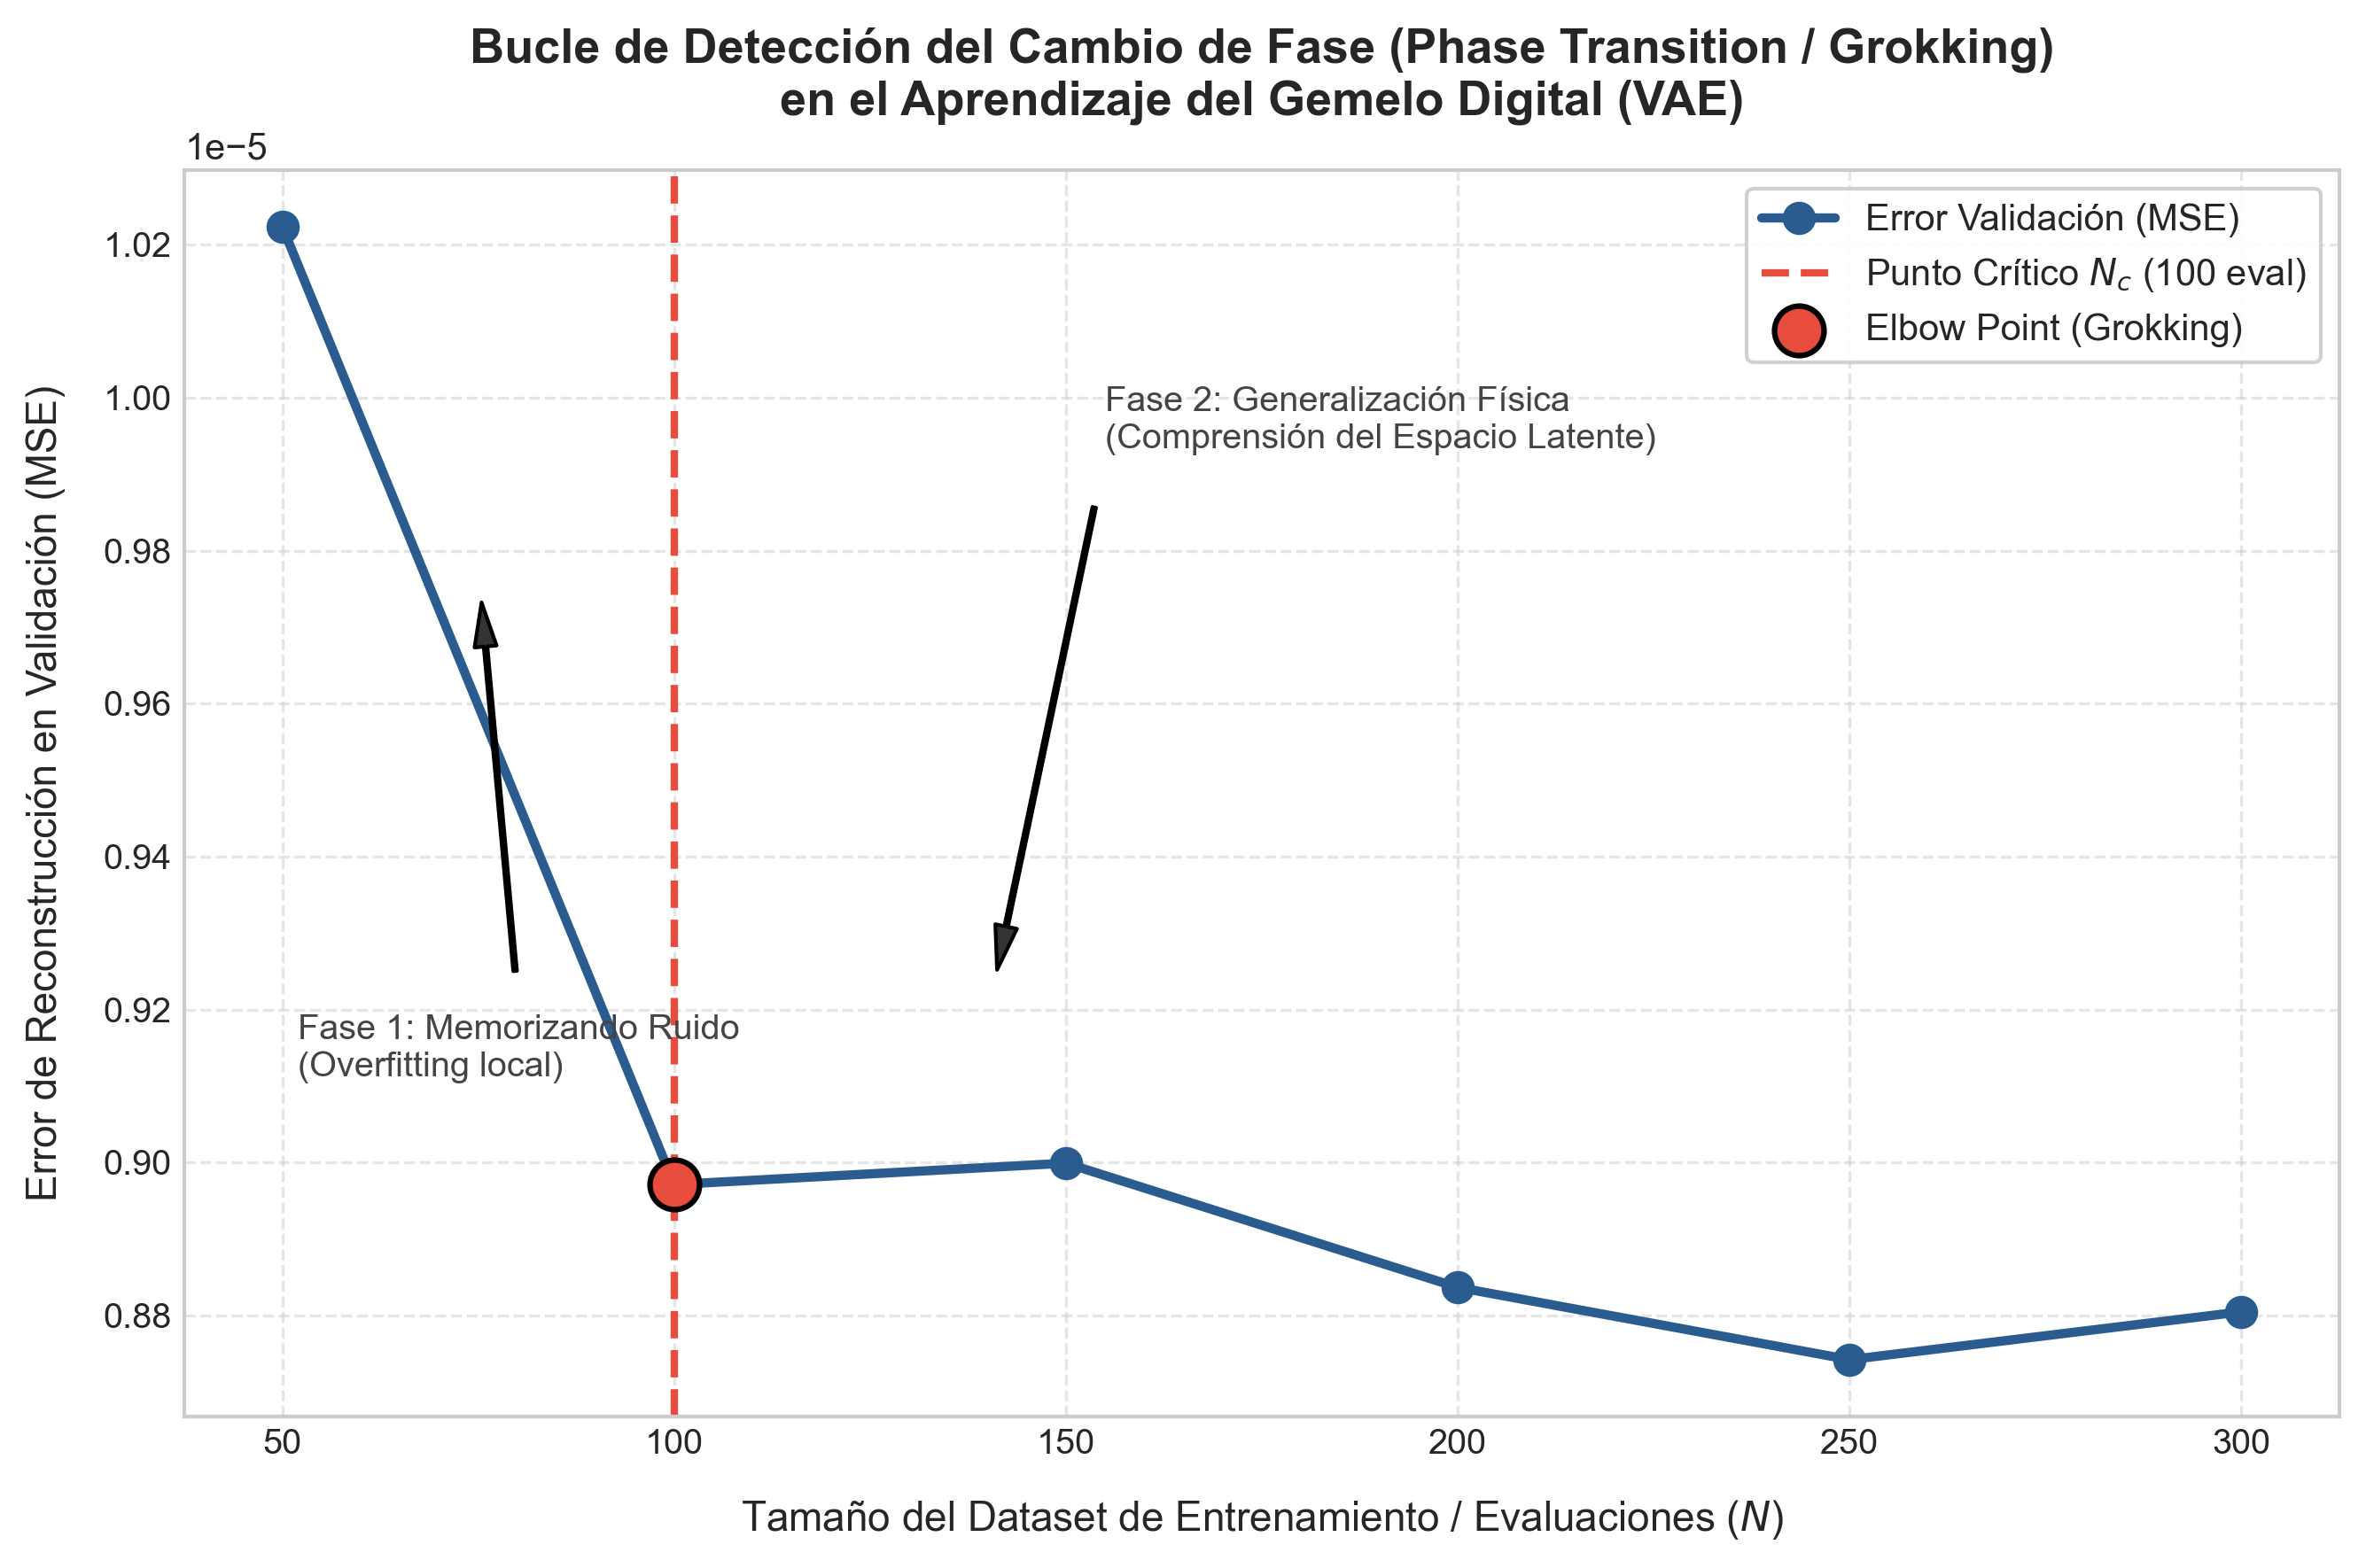
\includegraphics[width=0.85\textwidth]{../../Figuras/phase_transition_grokking}
    \caption{Curva experimental del error de reconstrucción en validación vs. tamaño de dataset $N$. La línea discontinua marca la transición crítica en $N_c = 100$.}
    \label{fig:grokking}
\end{figure}

Como se observa en la Figura \ref{fig:grokking}, existe un cambio de pendiente abrupto (codo) en la vecindad de $N = 100$. 
\begin{itemize}
    \item \textbf{Fase 1 ($N < 100$):} El error de reconstrucción es más alto porque el modelo cuenta con muy pocos ejemplos y memoriza las peculiaridades ruidosas del dataset de entrenamiento, fallando al generalizar en datos no vistos.
    \item \textbf{Fase 2 ($N \ge 100$):} El error se reduce drásticamente y se estabiliza. En este régimen, el VAE ha decodificado correctamente las correlaciones espaciales continuas del haz de iones, operando bajo un entendimiento generalizado de la variedad de datos.
\end{itemize}

\section{Densificación Local de la Variedad por Micro-Perturbación}
Dado que el espacio de voltajes posibles es de 8 dimensiones y el volumen donde el haz llega enfocado al detector es muy estrecho, el muestreo puramente aleatorio es ineficiente. Para enriquecer localmente el dataset sin gastar en simulaciones estériles de transmisión nula, se implementó un proceso de densificación.

\subsection{Algoritmo de Perturbación Local}
La lógica del proceso se describe a continuación:
\begin{enumerate}
    \item \textbf{Filtrado:} Se seleccionaron los $K=5$ mejores voltajes basándose en su tasa de transmisión (en este caso, aquellas configuraciones que resultaron en impactos de iones positivos).
    \item \textbf{Perturbación Gaussiana:} Para cada una de estas $K$ configuraciones base $Y_k \in \mathbb{R}^8$, se generaron $M=10$ muestras de voltajes perturbados sumando ruido Gaussiano:
    \begin{equation}
        Y_{k, m}^{\text{nuevo}} = Y_k + \boldsymbol{\epsilon}_{k, m}, \quad \boldsymbol{\epsilon}_{k, m} \sim \mathcal{N}(\mathbf{0},\, \sigma^2 \mathbf{I})
    \end{equation}
    Se seleccionó una desviación estándar de ruido de $\sigma = 20.0\text{ V}$, permitiendo explorar la frontera inmediata de las mejores configuraciones iónicas.
    \item \textbf{Recorte Físico (Clipping):} Para cada nuevo voltaje propuesto, se aplicó un filtro de acotamiento para mantener los voltajes resultantes en el límite de operación del laboratorio:
    \begin{equation}
        V_{i} = \max(-1000.0, \min(V_{i}, 1000.0))
    \end{equation}
\end{enumerate}

El código modular que implementa esta lógica se expone a continuación:
\begin{lstlisting}[language=Python]
def generar_perturbaciones_locales(mejores_voltajes, num_perturbaciones, sigma):
    base_voltages = mejores_voltajes[voltage_cols].values
    K, d = base_voltages.shape
    new_voltages = []
    
    for i in range(K):
        v_base = base_voltages[i]
        for _ in range(num_perturbaciones):
            ruido = np.random.normal(0, sigma, size=d)
            v_nuevo = v_base + ruido
            v_nuevo = np.clip(v_nuevo, -1000.0, 1000.0)
            new_voltages.append(v_nuevo)
            
    return pd.DataFrame(new_voltages, columns=voltage_cols)
\end{lstlisting}

\subsection{Dataset Densificado para SIMION}
Como resultado, el pipeline generó $K \times M = 50$ configuraciones de voltajes densificadas, almacenadas en la carpeta de estudiante bajo el archivo \texttt{voltajes\_perturbados\_lhs.csv}. Evaluar estas 50 perturbaciones en SIMION permitirá acumular perfiles de haz con impactos positivos, dotando al emulador Forward de una precisión muy alta en el modelado del haz enfocado.

\section{Conclusión}
La implementación de las modificaciones propuestas robustece la arquitectura del Gemelo Digital. La detección del cambio de fase permite dimensionar de manera informada el tamaño óptimo de dataset para la compresión latente ($N \ge 100$), mientras que la generación de micro-perturbaciones locales enriquece la base de entrenamiento del regresor, protegiéndolo contra la escasez de señal informativa.

\end{document}
